\documentclass[tikz,border=10pt]{standalone}
\usepackage{amsmath}
\usetikzlibrary{shapes.geometric, positioning} % Include positioning library

\begin{document}

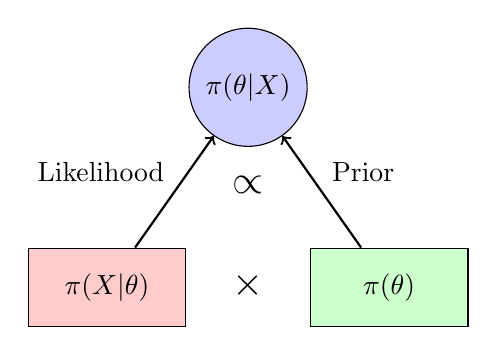
\begin{tikzpicture}
    % Posterior: \pi(\theta|X)
    \node[draw, circle, fill=blue!20, minimum size=1.5cm, align=center] (posterior) {$\pi(\theta | X)$};

    % Likelihood: \pi(X|\theta)
    \node[draw, rectangle, fill=red!20, minimum width=2cm, minimum height=1cm, align=center, below left=1.5cm and .25cm of posterior] (likelihood) {$\pi(X | \theta)$};

    % Prior: \pi(\theta)
    \node[draw, rectangle, fill=green!20, minimum width=2cm, minimum height=1cm, align=center, below right=1.5cm and .25cm of posterior] (prior) {$\pi(\theta)$};

    % Proportional sign
    \node[draw=none, align=center, below=0.25cm of posterior] (proportional) {\Large $\propto$};

    % Multiplication sign
    \node[draw=none, align=center, below=.75cm of proportional] (multiply) {\Large $\times$};

    % Arrows connecting components
    \draw[->, thick] (likelihood) -- node[midway, above left] {Likelihood} (posterior);
    \draw[->, thick] (prior) -- node[midway, above right] {Prior} (posterior);
\end{tikzpicture}

\end{document}
